\documentclass{beamer}

\usepackage{beamerthemesplit}
\usepackage{verbatim}

\usetheme{Pittsburgh}
%\usecolortheme{seagull}
%\usecolortheme{seahorse}
\usecolortheme{beaver}

\usefonttheme{serif}

%\DeclareGraphicsExtensions{.pdf,.png,.jpg}

\newcommand{\snT}{$(S/N)_{\textrm{size}}$}
%\newcommand{\snT}{$\left( \frac{S}{N}\right)_{\textrm{size}}$}
\newcommand{\snflux}{$(S/N)_{\textrm{flux}}$}
%\newcommand{\snflux}{$\left( \frac{S}{N}\right)_{\textrm{flux}}$}

\newcommand{\lensfit}{\texttt{LENSFIT}}
\newcommand{\numba}{\texttt{Numba}}
\newcommand{\python}{\texttt{Python}}
\newcommand{\ngmix}{\texttt{ngmix}}
\newcommand{\shear}{{\bf g}}

\title{Bayesian Shear Estimation}
\author{Erin Sheldon}
\institute{Brookhaven National Laboratory}

% http://texblog.net/latex-archive/plaintex/beamer-footline-frame-number/
% to add the page (frame ) number and not screw up the bottom line
% works for split themes?
\expandafter\def\expandafter\insertshorttitle\expandafter{%
      \insertshorttitle\hfill%
        \insertframenumber\,/\,\inserttotalframenumber}


\begin{document}

%\frame{\titlepage}

\section{Dark Energy Survey}

\frame
{
    \frametitle{Dark Energy Survey (DES)}

    \fontsize{9}{0.8\baselineskip}
    \begin{columns}
        \begin{column}{0.5\textwidth}    
            \begin{itemize}
                \item Imaging survey of 5000 square degrees in the 
                    southern sky (CTIO) through 5 optical filters.
                \item Study Dark Energy using weak lensing, galaxy clusters, supernovae
                    and large scale structure.
                \item First Light Fall 2012
                \item Survey Start Aug. 31 2013
                \item Erin Sheldon {\bf associate member and builder}; data rights for
                    himself, postdoc, students.
                \item Anders Plazas postdoc working on characterization of detector
                    effects and weak lensing.
            \end{itemize}
        \end{column}
        \begin{column}{0.5\textwidth}
            \includegraphics[width=\textwidth]{ctio_blanco_crew_2013Oct-19-contrast.jpg}
        \end{column}
    \end{columns}
}
\frame
{
    \frametitle{Oct. 2013 DES Observing Run}

    \includegraphics[width=\textwidth]{ctio_blanco_crew_2013Oct-13-contrast.jpg}
}
\frame
{
    \frametitle{Sept. 2013 DES Observing Run}

    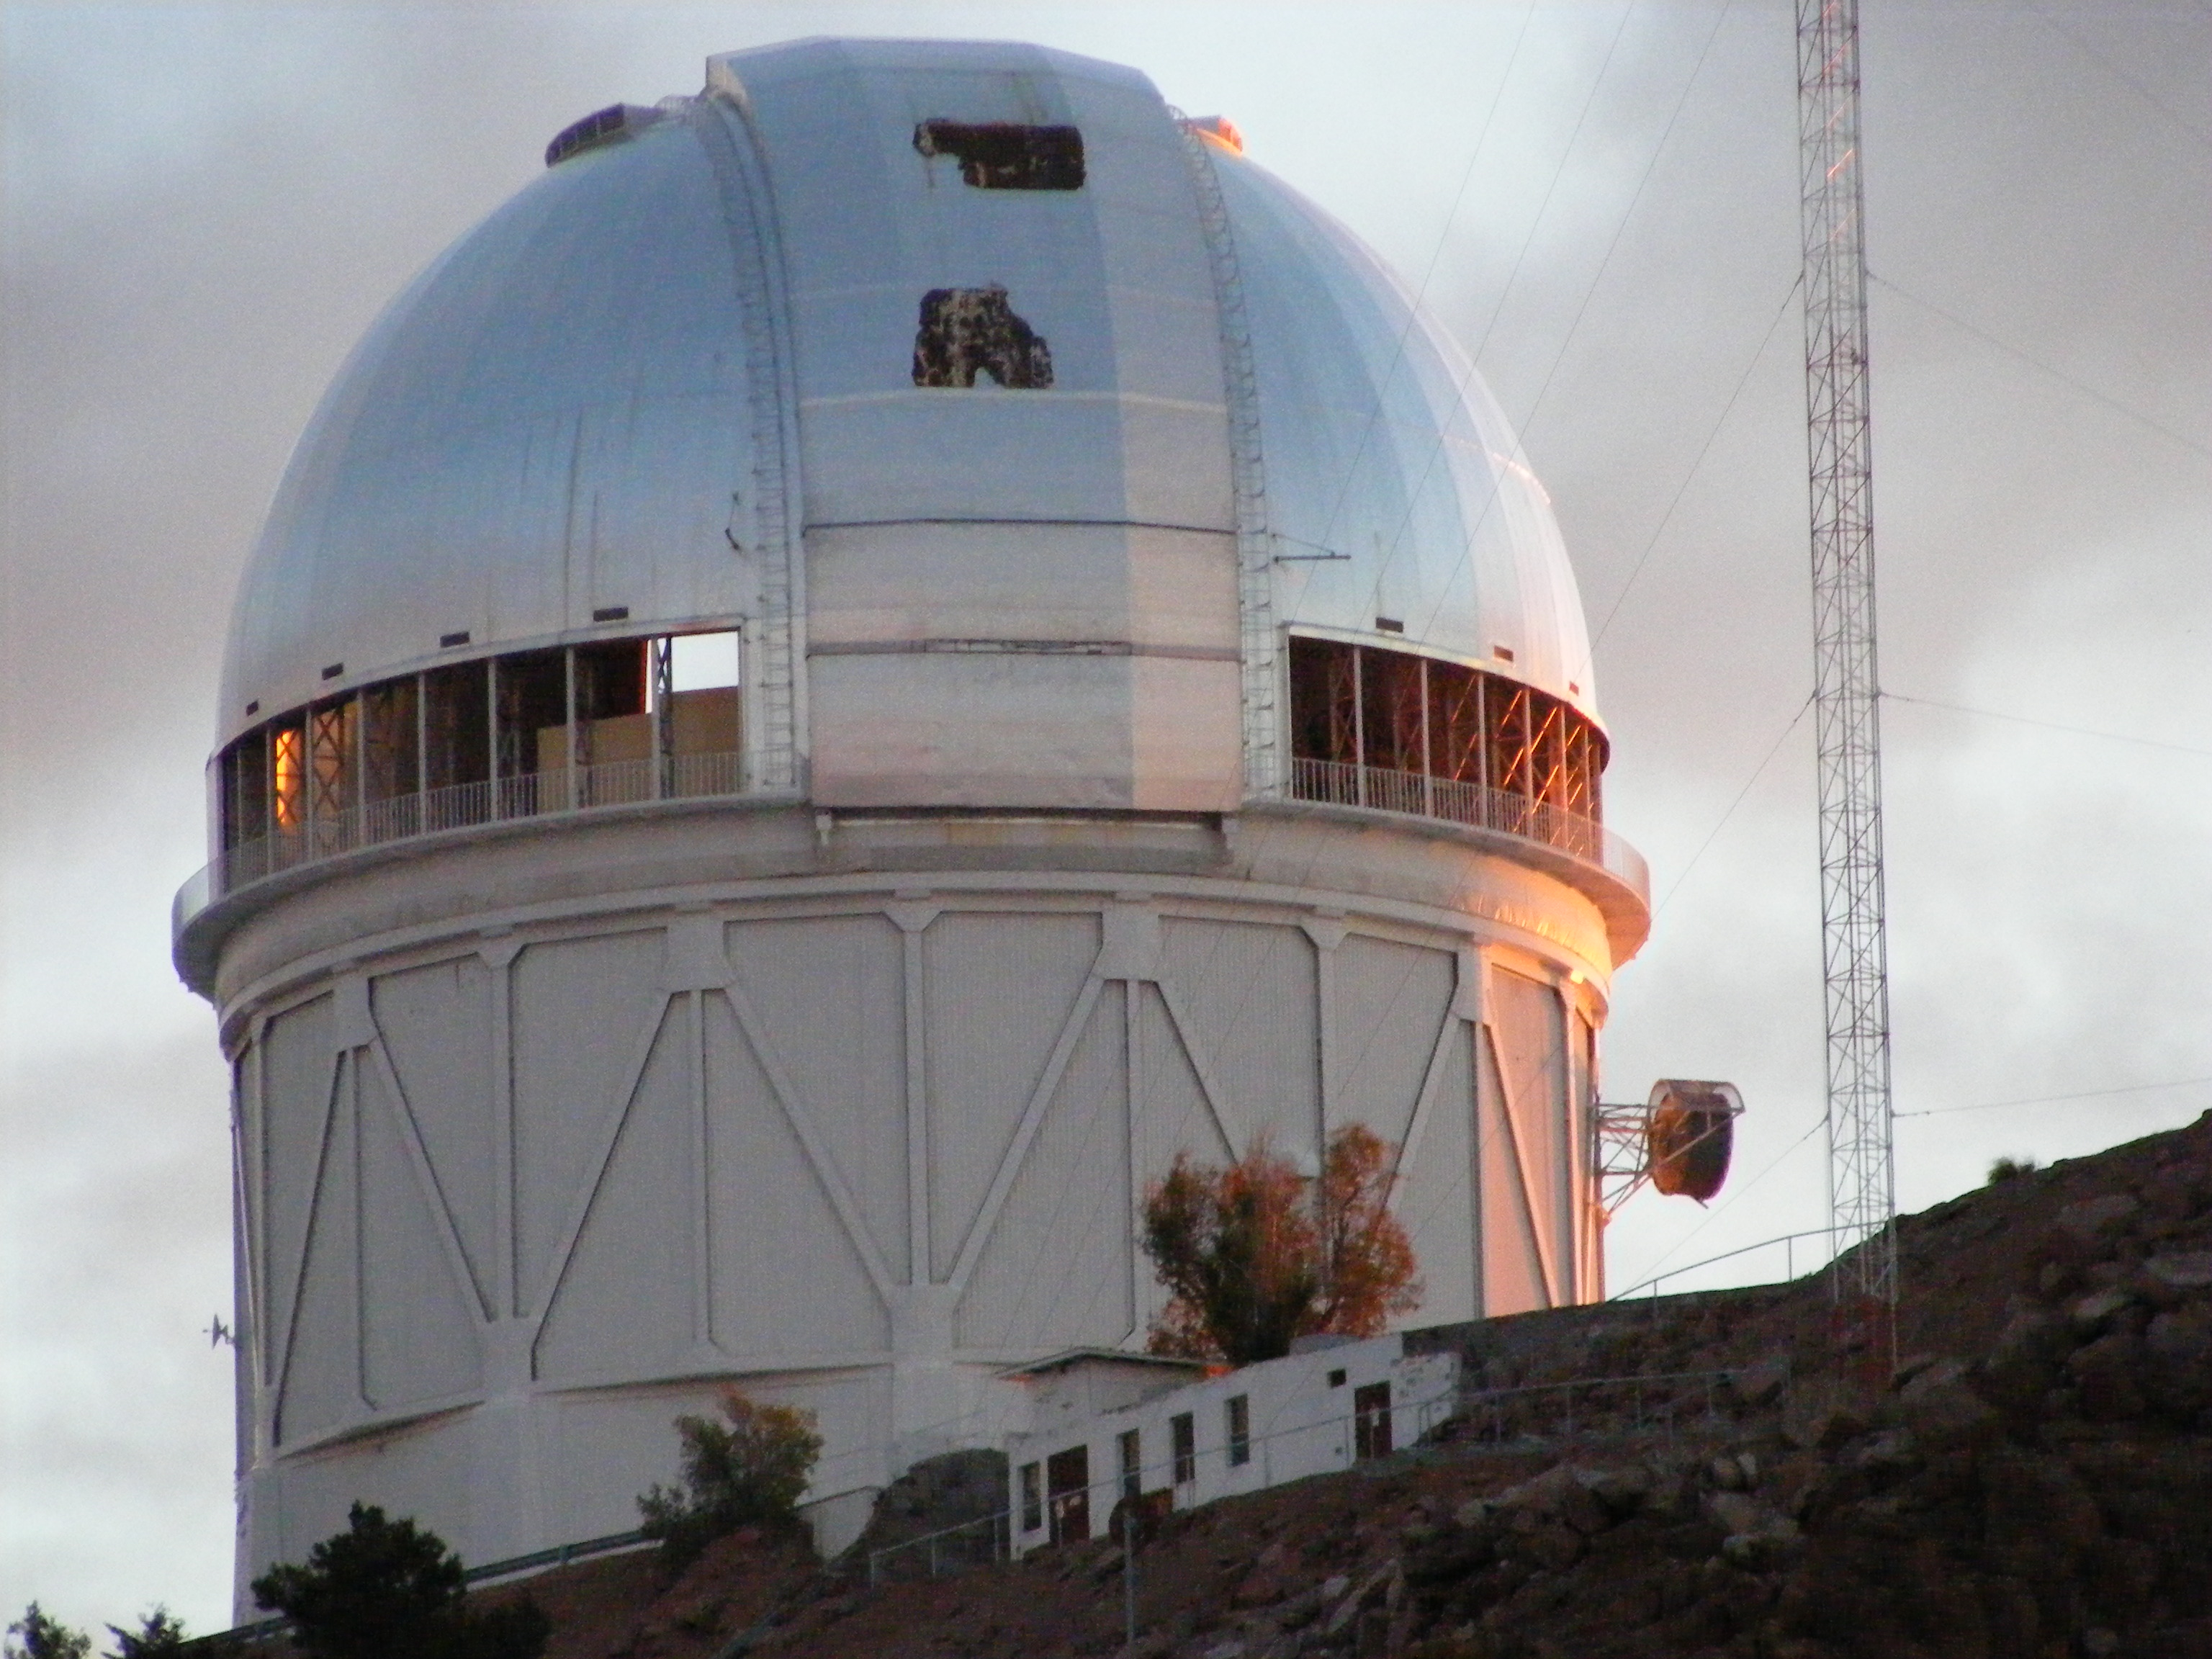
\includegraphics[width=0.5\textwidth]{plazas-blanco-ctio.jpg}
    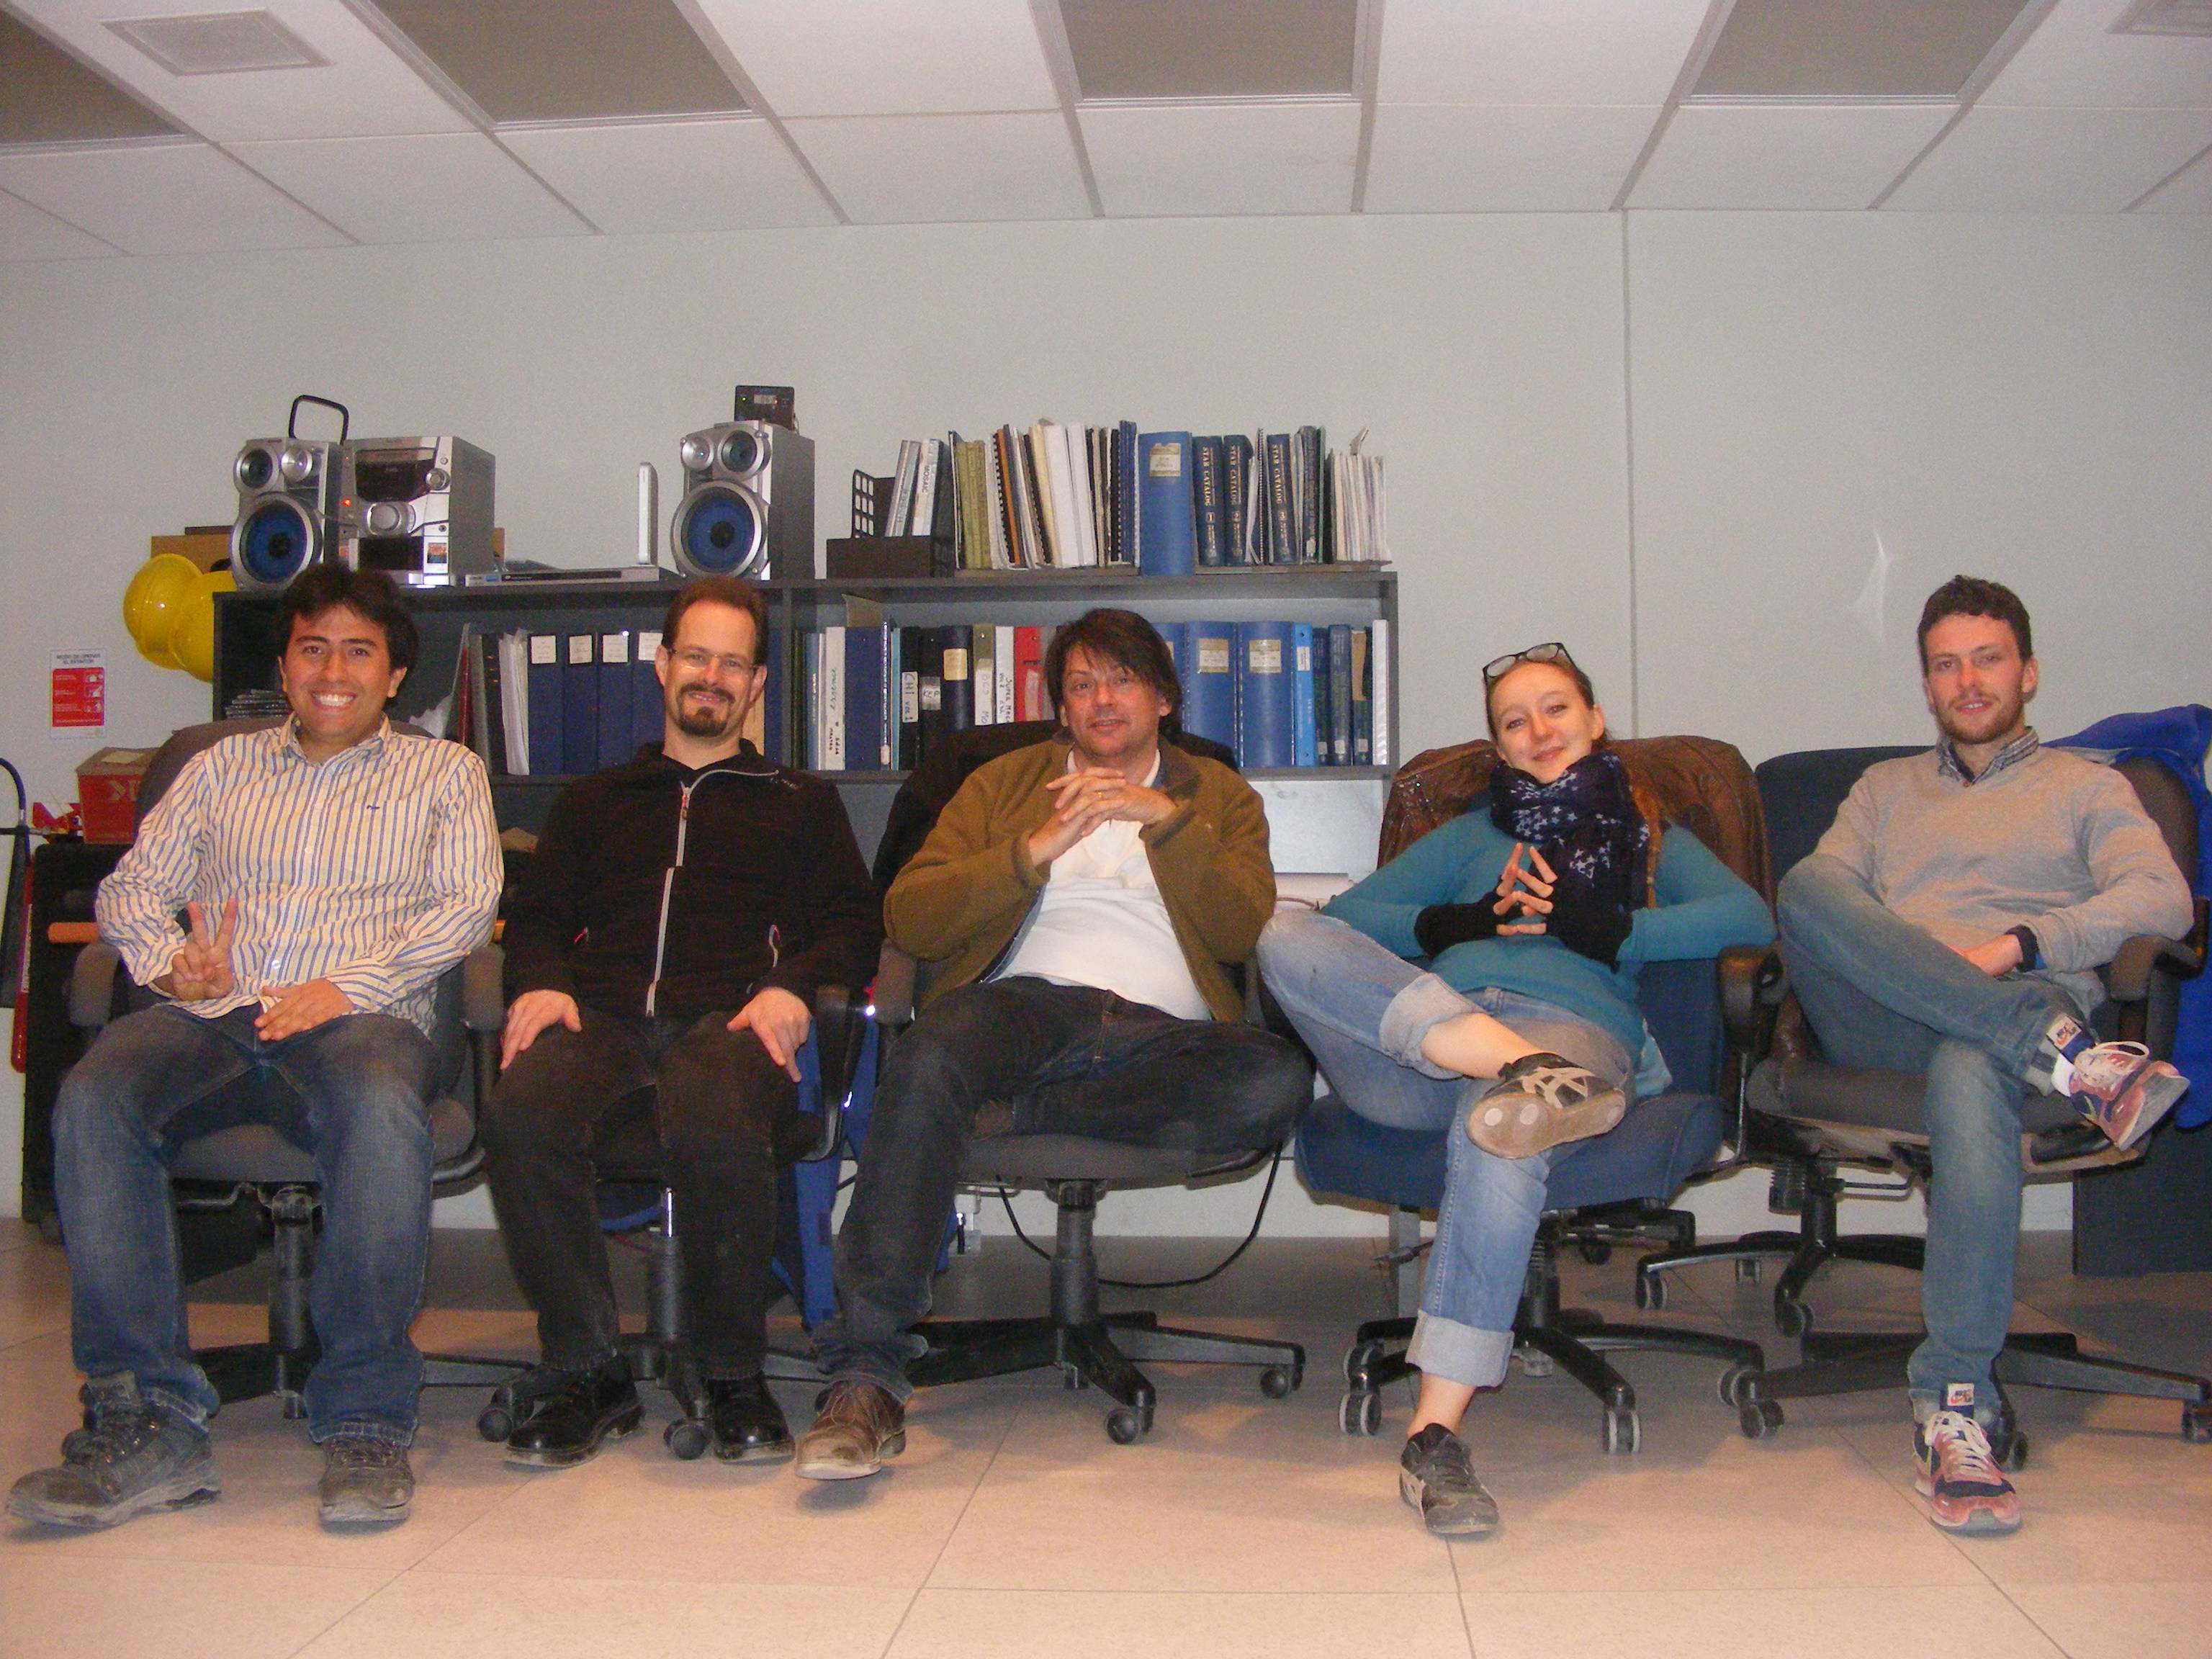
\includegraphics[width=0.5\textwidth]{plazas-group-ctio.jpg}
}


\frame
{
    \frametitle{DES Contributions from Erin Sheldon}

    \fontsize{9}{0.9\baselineskip}
    \begin{itemize}

        \item DES data is multi-epoch: the same area of sky is observed
            multiple times during the survey.  Early data has $\sim$10 epochs.
            Optimal processing for lensing involves a full joint fit to all
            data, no coadding.

        \item Erin Sheldon built infrastructure to facilitate transparent
            processing DES multi-epoch data.  All lensing pipelines now use
            this infrastructure.

        \item Erin Sheldon is finalizing a Bayesian shear measurement pipeline,
            based on recent theoretical developments (Bernstein \& Armstrong).
            This method meets DES requirements for lensing calibrations (and indeed
            LSST as well).  See next slide.  This pipeline is running on DES data.

        \item Erin Sheldon and Peter Melchior built the ``Exposure Checker'', a
            {\it crowdsourcing} project that allows scientists to examine exposures
            from DES on the web, mark them for defects (or awesomeness),
            and easily report findings.

    \end{itemize}
}

\frame
{
    \frametitle{Bayesian Lensing Shear Measurement}

    \begin{columns}
        \begin{column}{0.4\textwidth}
            \begin{itemize}

                \item Figure: Fractional error in the shear for simulated galaxies
                    (exp,dev profiles) near smallest usable {\it observed} size
                    fwhm/fwhm$_{\textrm{psf}}$ = 1.2.

                \item Light Grey: DES requirements
                \item Dark Grey: LSST requirements
            \end{itemize}
        \end{column}
        \begin{column}{0.6\textwidth}
            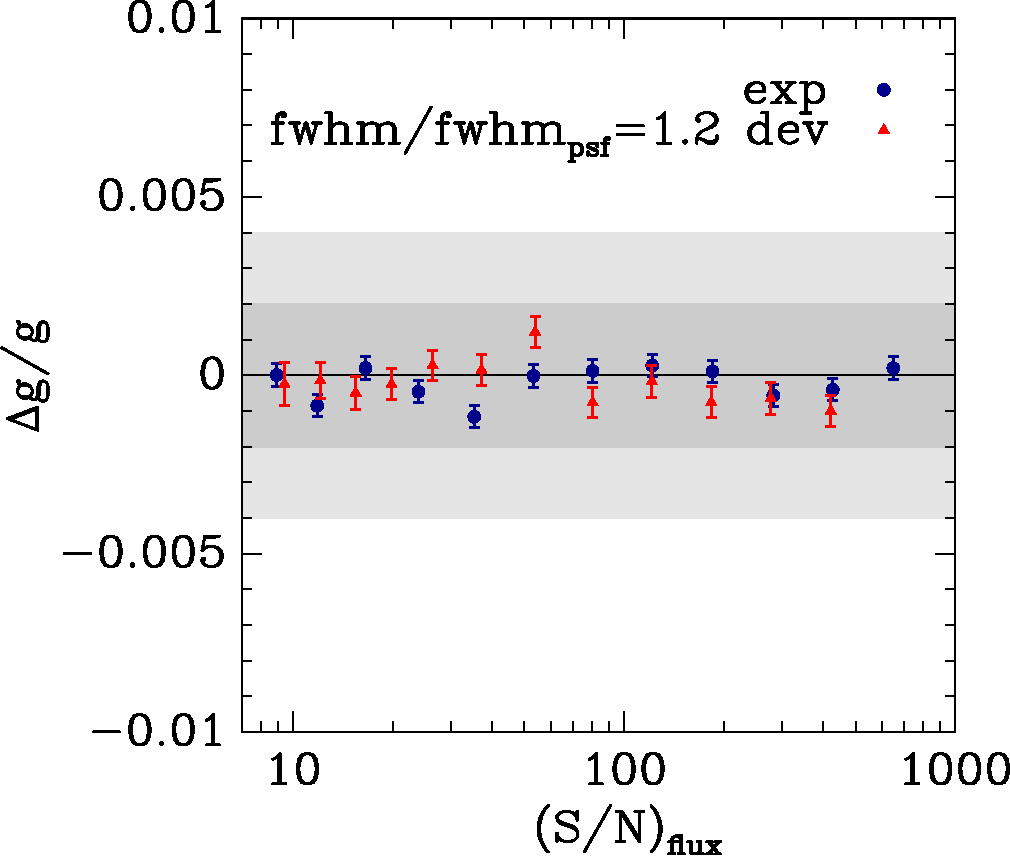
\includegraphics[width=\textwidth]{ngmix-flux-s2n-sigrat-20.pdf}
            \newline

            {\tiny Implementation of recent theoretical work by Bernstein \&
             Armstrong.\par}

        \end{column}
    \end{columns}

}

\frame
{
    \frametitle{DES Detector Characterization: Andres Plazas}

    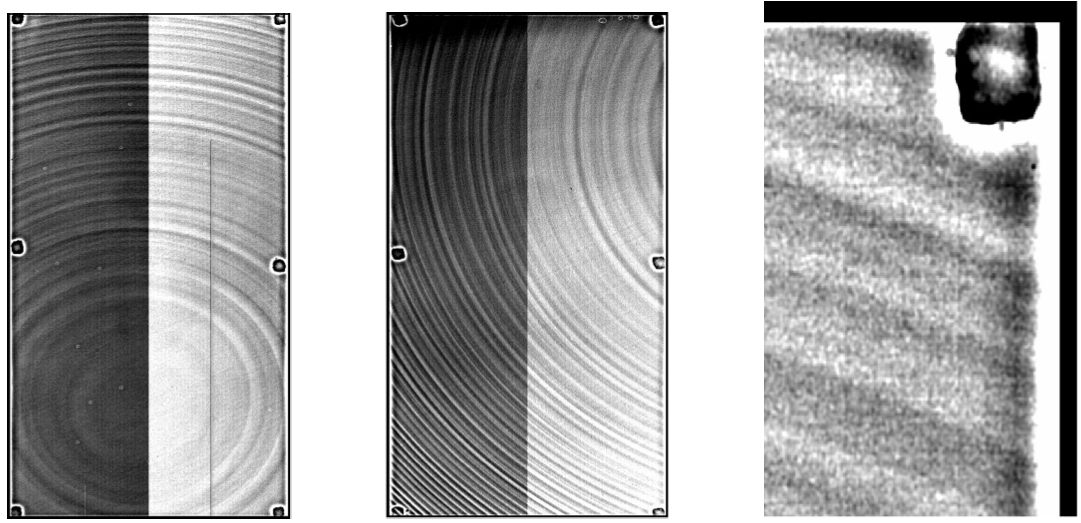
\includegraphics[width=\textwidth]{flats.png}
    \newline

    \begin{center}
        Tree rings and tape bumps in a flat field image.
    \end{center}
} 
\frame
{
    \frametitle{DES Detector Characterization: Andres Plazas}

    \fontsize{9}{0.7\baselineskip}
    \begin{columns}
        \begin{column}{0.4\textwidth}
            \begin{itemize}

                \item Tree-rings are features in the CCDs that occur during
                    fabrication.  Variations in doping produces a spurious
                    transverse electric field, changing the effective location
                    and area of each pixel.

                \item In typical image reduction the data are divided by these
                    calibration frames, but this is incorrect : our
                    measurements indicate this introduces large systematic
                    errors.

                \item We measure these instrumental signatures and produce
                    models that fit the data well.

            \end{itemize}
        \end{column}
        \begin{column}{0.6\textwidth}
            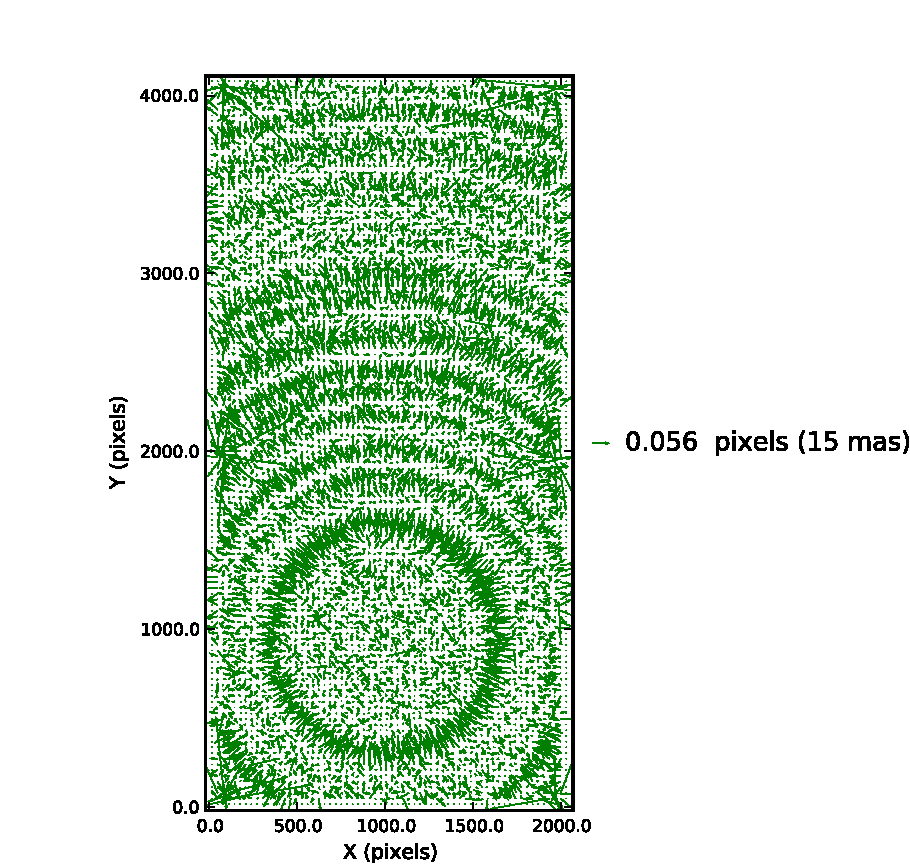
\includegraphics[width=\textwidth]{N22_astrometric_single-crop.pdf}
            \newline

            {\tiny Astrometric residuals from polynomial model caused by
            the ``tree rings''. \par}


        \end{column}
    \end{columns}


}

\frame
{
    \frametitle{DES Detector Characterization: Andres Plazas}

    \begin{center}
    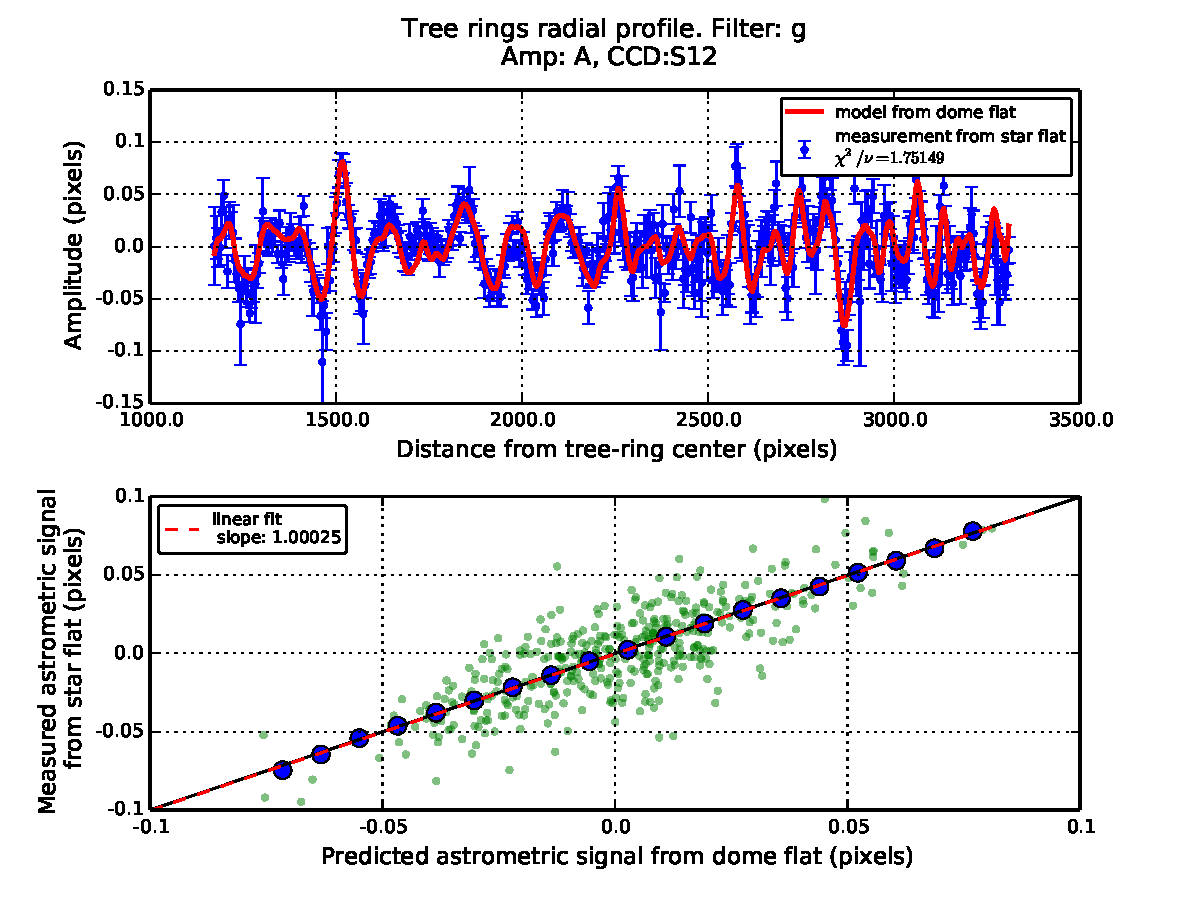
\includegraphics[width=0.7\textwidth]{astrometric_residuals_vs_model_S12.pdf}
\end{center}

    {\small 
        \begin{itemize}
            \item Astrometric residuals binned in radius from center of tree ring.
            \item Prediction from model fit to the flat field matches well.
        \end{itemize}
    }
}



\end{document}
